\documentclass{pizzablatt}

\geometry{tmargin=1.5cm,bmargin=1.0cm,lmargin=2.60cm,rmargin=2.60cm}

\setlength{\aufgabenskip}{1.0em}

\begin{document}

\setlength{\unitlength}{1cm}
\begin{picture}(0,0)
  \put(14,-11){\vbox{%
    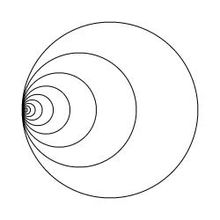
\includegraphics[scale=0.4]{hawaiian-earrings.png} \\
    \hspace*{1em}\tiny Hawaiische Ohrringe
  }}
\end{picture}

\maketitle{1}{Pizzaseminar zur Knotentheorie}{4. September 2013}

\begin{aufgabe}{Konkrete Knoten und Verschlingungen}
\begin{enumerate}
\item Zu welchem bekannten Knoten ist der links abgebildete Knoten äquivalent?
\item Eine Verschlingung heißt genau dann \emph{zerlegbar}, wenn sich ihre
Komponenten so deformieren lassen, dass sie auf verschiedenen Seiten einer
Ebene des dreidimensionalen Raums liegen. Ist die rechts abgebildete Verschlingung
zerlegbar?
\end{enumerate}
\vspace{-1em}

\begin{center}
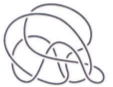
\includegraphics{knoten-1}
\hspace{3em}
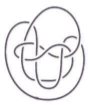
\includegraphics{knoten-2}
\end{center}
\end{aufgabe}

\begin{aufgabe}{Triviale Knoten}
\begin{enumerate}
\item Ist jeder Knoten mit genau vier Eckpunkten trivial?
\item Ist jeder Knoten mit genau fünf Eckpunkten trivial?
\item Zeige, dass jeder Knoten mit genau zwei Überkreuzungen trivial ist.
\end{enumerate}
\end{aufgabe}

\begin{aufgabe}{Abänderung von Projektionen}
Zeige, dass durch geeignete Abänderung der Überkreuzungen in Unterkreuzungen
oder umgekehrt aus jeder Projektion eines Knotens eine Projektion des Unknotens
erzeugt werden kann.
\end{aufgabe}

\begin{aufgabe}{Knoten auf Tori}
\begin{enumerate}
\item Welche Knoten gibt es auf dem zweidimensionalen Torus (der
Donutoberfläche oder dem zweidimensionalen Asteroids-Spielfeld)?
\item[b)$^\star$] Welche Knoten gibt es auf dem dreidimensionalen Torus? Diesen kann man
sich als ein dreidimensionales Asteroids-Spielfeld vorstellen, also als ein
Zimmer, in dem man wieder links herauskommt, wenn man gegen die rechte Wand
läuft, und genauso mit vorne/hinten und unten/oben.
\end{enumerate}
\end{aufgabe}

\begin{aufgabe}{Ein Spezialfall des Satzes von Seifert und van Kampen}
Seien~$X$ und $Y$ offene und wegzusammenhängende Teilmengen
eines topologischen Raums. Sei ferner der Schnitt~$X \cap Y$ nichtleer und
wegzusammenhängend. Zeige, dass wenn~$X$ und~$Y$ einfach zusammenhängend
sind, dann auch~$X \cup Y$ einfach zusammenhängend ist. \emph{Schon ein
informaler Beweis ist interessant.}

Dabei heißt ein Raum~$A$ genau dann \emph{wegzusammenhängend}, wenn es zu je zwei
Punkten~$x,y \in A$ eine stetige Abbildung~$\gamma : [0,1] \to A$
mit~$\gamma(0) = x$ und~$\gamma(1) = y$ gibt. Ein Raum~$A$ heißt genau dann
\emph{einfach zusammenhängend}, wenn er wegzusammenhängend ist und jede
Schleife nullhomotop ist (sich also zu einer konstanten Punktkurve homotopieren
lässt).
\end{aufgabe}

\begin{aufgabe}{Hawaiische Ohrringe}
Sei~$X \subseteq \RR^2$ die Vereinigung der Kreislinien mit Mittelpunkten~$(1/n,
0)$ und Radien~$1/n$, $n \geq 1$ (siehe Skizze oben). Gib explizit eine stetige
Abbildung~$\gamma : [0,1] \to X$ an, die als Bild ganz~$X$ hat, und weise ihre
Stetigkeit nach.
\end{aufgabe}

\end{document}
